\documentclass[conference]{IEEEtran}
\IEEEoverridecommandlockouts
% The preceding line is only needed to identify funding in the first footnote. If that is unneeded, please comment it out.
\usepackage{cite,comment,hyperref}
\usepackage{amsmath,amssymb,amsfonts}
\usepackage{tikz}
\usepackage{algorithmic}
\usepackage{graphicx}
\usepackage{textcomp}
\usepackage{xcolor}
\usetikzlibrary{calc,shapes}
\def\BibTeX{{\rm B\kern-.05em{\sc i\kern-.025em b}\kern-.08em
    T\kern-.1667em\lower.7ex\hbox{E}\kern-.125emX}}
    
\begin{document}

\title{Towards realizing a cloud-native B5G mobile core architecture}


\author{\IEEEauthorblockN{Quang Tung Thai, Namseok Ko}
\IEEEauthorblockA{\textit{Network Research Division} \\
\textit{ETRI}\\
Daejeon, Republic of Korea \\
\texttt{\{tqtung, nsko\}@etri.re.kr}}

}

\maketitle

\begin{abstract}

The 5G mobile core moved away from a monolithic design toward a service based
	architecture as the network now being composed of small interacting
	software components so called network functions. The change is to
	enable horizontal scalability and flexibility in network deployments to
	meet various vertical use cases of stringent requirements. Going beyond
	5G, it is clear that mobile core networks will base on the maturing
	cloud-native technology with network functions being deployed in
	multiple distributed clouds. This paper discusses limitations of the
	current core architecture with a forward looking to its cloud-native
	realization. In order to completely adopt the cloud-native trend, the
	architecture should be restructured to enable a clear separation
	between development and deployment of mobile network services.
	Following this vein, we make a holistic architectural change to the
	core by moving some of it parts into an integration fabric layer. We
	discuss how the fabric is designed and its benefits to the development
	of the beyond 5G core network.

\end{abstract}

\begin{IEEEkeywords}
B5G, SBA, service mesh, integration fabric, service discovery
\end{IEEEkeywords}

\section{Introduction}

The 5G mobile network was designed on a premise that it is to support various
types of services with very different performance requirements on a common
physical network infrastructure. Meeting this new challenge demands a paradigm
shift. A fundamental change in 5G core network design is abandoning monolithic
system in favors of a Service Based Architecture (SBA)\cite{5g}.  With this new
approach, the core network is decomposed into software components of different
functionalities. These so called network functions (NF) expose services in the
form of restful APIs.  Signalling procedures in the core network involve
interacting of the network functions through requesting these services.
Decomposing the network into small software components enables flexible and
scalable deployments. The network can be provisioned and managed with
fine-grain controls. 

Following this path, it is foreseeable that the future core network will be
cloud-native oriented\cite{telco}. Many software-based network functions will
be containerized and deployed at multiple clouds: at the core, at the edge of
the network or at premise of verticals. Cloud technology enables the ability to
share infrastructure resources: service workloads can be allocated dynamically
to meet the service level agreements of existing and future demanding use
cases. Adopting cloud-native facilitated automation and continuous
innovation/continuous deployment will help network operators to reduce time to
market, respond sooner to customer demands.

However, the current architecture is far from cloud-native friendly.  In fact,
except for a few proof-of-concept small-scale examples \cite{kube5g}, we have
not seen any attempt to demonstrate a large-scale deployment of 5G core on
Kubernetes \cite{ku8}, the de-factor container orchestration platform. One
reason is that the design was being made with a whole system oriented mindset.
It has not taken advantage of maturing features of existing cloud-native
platforms.  Instead, two separated issues was considered at the same time: on
one hand, there are network components to handle signaling procedures of mobile
applications; on the other hand, there are network components to enable
deployments with scalability and flexibility. The second issue concerns with
the discovery and selection of services in deployments.  This has been
addressed thoroughly using a service mesh \cite{mesh} in cloud-native
platforms. Fitting the 5G core into a cloud platform, therefore, still looks
very peculiar.


In this work, we make a very first attempt to analyze limitations of the
current 5G core architecture towards complex large-scale multi-cluster
cloud-native deployments, which are the very common scenarios going beyond 5G.
We push for a architectural holistic changes to embrace the fundamental
principal of the cloud-native development philosophy: a clear separation
between service development and service deployment. That is, developers should
only focus on the business logic to enable the application functionalities
without concerning about deployment matters including scalability, reliability
and observability.  We propose moving some network functions into a separated
layer called integration fabric. The fabric takes care of service registration,
discovery and selection and exposes a unified interface to the business layer
of network functions. This change will not only simplify the implementation of
network functions but also open up the possibility of integration new types of
services into an existing network.


The remaining of the paper is organized as follows. Section \ref{sec:analysis}
provides an analysis of current mobile core network architecture to address its
limitations when being deployed in cloud-native platforms. In Section
\ref{sec:arch}, we introduce the concept of integration fabric and present how
we design it. Within the section, we also explain the interface between the
fabric and network functions, and how service registration and discovery can be
implemented in a distributed manner. The Section \ref{sec:conc} summaries our
work with a discussion on the advantage of the proposed fabric.


\section{Analysis of the current architecture \label{sec:analysis}}

\subsection{Service discovery and selection \label{sec:disc}}

\begin{figure}
\begin{center}
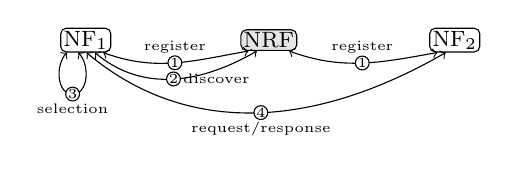
\begin{tikzpicture}[nf/.style={draw, rounded corners=2pt, fill=white, inner sep=1pt,font=\footnotesize},
lab/.style={circle, draw, fill=white,minimum width=5pt,inner sep=0}]
	\node[nf] at (0,0) (nf1) {NF$_1$};
	\node[nf, fill=black!10] at ([xshift=2cm]nf1.east) (nrf) {NRF};
	\node[nf] at ([xshift=2cm]nrf.east) (nf2) {NF$_2$};
	\draw[<->] ([xshift=-3pt]nf1.south east) to[out=-20,in=190] coordinate (l1) ([xshift=3pt]nrf.south west);
	\draw[<->] ([xshift=-3pt]nrf.south east) to[out=-20,in=190] coordinate (l2) ([xshift=3pt]nf2.south west);
	\draw[<->] ([xshift=-6pt]nf1.south east) to[out=-40,in=210] coordinate (l3) ([xshift=6pt]nrf.south west);
	\draw[<->] ([xshift=-9pt]nf1.south east) to[out=-40,in=210] coordinate (l4) ([xshift=6pt]nf2.south west);
	\draw[<->] ([xshift=-12pt]nf1.south east) to[out=-45,in=0] ([xshift=-14pt,yshift=-15pt]nf1.south east) coordinate (l5)  to[out=180,in=-135] ([xshift=-16pt]nf1.south east);
	\node[lab] at (l1) {\tiny 1};
	\node[lab] at (l2) {\tiny 1};
	\node[lab] at (l3) {\tiny 2};
	\node[lab] at (l5) {\tiny 3};
	\node[lab] at (l4) {\tiny 4};

	\node[below] at (l4) {\tiny request/response};
	\node[right] at (l3) {\tiny discover};
	\node[above] at (l2) {\tiny register};
	\node[above] at (l1) {\tiny register};
	\node[below] at (l5) {\tiny selection};
\end{tikzpicture}
	\caption{Service registration and discovery in TS 23.501 release
	15\cite{rel15}\label{fig:regdisc}}
\end{center}
\end{figure}

In the SBA, control plane of 5G core network consist of many network functions.
Each may fulfil certain functionality. A signalling procedure to serve an User
Terminal (UE) usually consists of a chain of communications among NFs; each may
process some steps of the procedure. One NF (consumer) may request a service from
another NF (producer) to fulfil its functionality. A producer may serve
multiple services to its consumers.

In a simple deployment, NFs can be configured manually to create static
connections among themselves. However, in large-scale dynamical deployments, they
should be discovered automatically. The NRF (Network Repository Function) is a
critical network function to enable the automation.  It is a centralized
service registry where other network functions can register their existences
and query for their peers' locations. 

Typically, when an NF is deployed, it registers its profile to the NRF so that
other NFs can request the services that it serves.  When a consumer wants to
request a service, it queries the NRF to look for a list of suitable
candidates. Once the list is received, it should select one of them to make a
request for the service. This interacting pattern is depicted on Figure
\ref{fig:regdisc}.

Although these steps look simple conceptually, its practical implementation
must use a load balancing algorithm for selection, and there must be a logic to
handle the case of failure (that is, the selected network function is failed).
It increases the complexity of deployment because of the differences in
implementations.  Subsequently it may lead to the vendor lock-in problem for
network operators.

\subsection{Service communication proxy}

\begin{figure}
	\begin{center}
		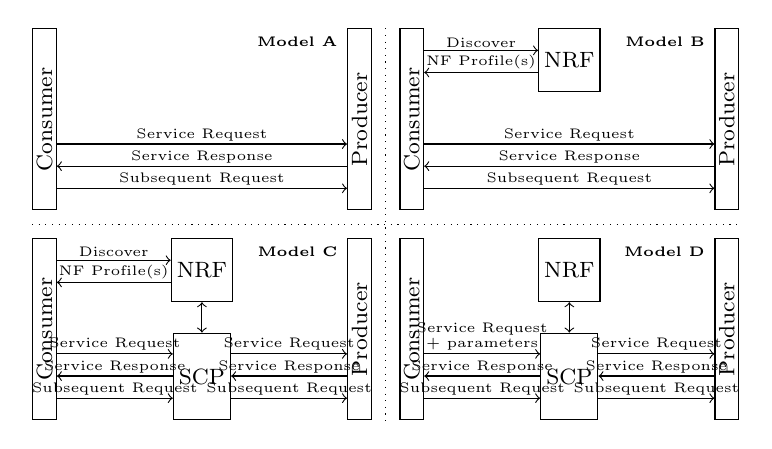
\begin{tikzpicture}[
			nf/.style={rectangle, draw, minimum width=0.3cm, minimum height=2.3cm, inner sep=2pt},
			linklab/.style={above,font=\tiny, inner sep=1pt},
			nrf/.style={rectangle,draw,minimum width=0.6cm, minimum height=0.8cm, inner sep=2pt,font=\footnotesize,align=center},
			scp/.style={rectangle,draw,minimum width=0.6cm, minimum height=1.1cm, inner sep=2pt,font=\footnotesize,align=center}
				]
			\def\w{4cm}
			\def\gap{10pt}
			\def\step{8pt}
			\node[nf] at (0,0) (c1) {};
			\node[nf] at ([xshift=\w]c1) (p1) {};
			\node[nf,below] at ([yshift=-\gap]c1.south) (c2) {};
			\node[nf] at ([xshift=\w]c2) (p2) {};

			\node[nf,right] at ([xshift=\gap]p1.east) (c3) {};
			\node[nf] at ([xshift=\w]c3) (p3) {};
			\node[nf,below] at ([yshift=-\gap]c3.south) (c4) {};
			\node[nf] at ([xshift=\w]c4) (p4) {};

			\foreach \i in {1,2,3,4} {
				\node[font=\footnotesize,rotate=90] at (c\i) {Consumer};			
				\node[font=\footnotesize,rotate=90] at (p\i) {Producer};			
			}

			\node[font=\tiny,left] at ([yshift=-5pt]p1.north west) {\textbf{Model A}};
			\node[font=\tiny,left] at ([yshift=-5pt]p3.north west) {\textbf{Model B}};
			\node[font=\tiny,left] at ([yshift=-5pt]p2.north west) {\textbf{Model C}};
			\node[font=\tiny,left] at ([yshift=-5pt]p4.north west) {\textbf{Model D}};

			%A
			\draw[->] ([yshift=\step]c1.south east) -- node[linklab] {Subsequent Request} ([yshift=\step]p1.south west);
			\draw[<-] ([yshift=2*\step]c1.south east) -- node[linklab] {Service Response} ([yshift=2*\step]p1.south west);
			\draw[->] ([yshift=3*\step]c1.south east) -- node[linklab] {Service Request} ([yshift=3*\step]p1.south west);
			%B
			\draw[->] ([yshift=\step]c3.south east) -- node[linklab] {Subsequent Request} ([yshift=\step]p3.south west);
			\draw[<-] ([yshift=2*\step]c3.south east) -- node[linklab] {Service Response} ([yshift=2*\step]p3.south west);
			\draw[->] ([yshift=3*\step]c3.south east) -- node[linklab] {Service Request} ([yshift=3*\step]p3.south west);
			
			\node[nrf,below] at ([xshift=0.5*\w]c3.north) (nrf3) {NRF};
			\draw[<-] ([yshift=-\step]nrf3.north west) -- node[linklab] {Discover} ([yshift=-\step]nrf3.north west -| c3.east);
			\draw[->] ([yshift=-2*\step]nrf3.north west) -- node[linklab] {NF Profile(s)} ([yshift=-2*\step]nrf3.north west -| c3.east);
			%C
			\node[nrf,below] at ([xshift=0.5*\w]c2.north) (nrf2) {NRF};
			\node[scp,above] at ([xshift=0.5*\w]c2.south) (scp2) {SCP};
			\draw[<->] (nrf2) -- (scp2);
			\draw[<-] ([yshift=-\step]nrf2.north west) -- node[linklab] {Discover} ([yshift=-\step]nrf2.north west -| c2.east);
			\draw[->] ([yshift=-2*\step]nrf2.north west) -- node[linklab] {NF Profile(s)} ([yshift=-2*\step]nrf2.north west -| c2.east);
			\draw[->] ([yshift=\step]c2.south east) -- node[linklab] {Subsequent Request} ([yshift=\step]scp2.south west);
			\draw[<-] ([yshift=2*\step]c2.south east) -- node[linklab] {Service Response} ([yshift=2*\step]scp2.south west);
			\draw[->] ([yshift=3*\step]c2.south east) -- node[linklab] {Service Request} ([yshift=3*\step]scp2.south west);

			\draw[->] ([yshift=\step]scp2.south east) -- node[linklab] {Subsequent Request} ([yshift=\step]p2.south west);
			\draw[<-] ([yshift=2*\step]scp2.south east) -- node[linklab] {Service Response} ([yshift=2*\step]p2.south west);
			\draw[->] ([yshift=3*\step]scp2.south east) -- node[linklab] {Service Request} ([yshift=3*\step]p2.south west);
			
			%D
			\node[nrf,below] at ([xshift=0.5*\w]c4.north) (nrf4) {NRF};
			\node[scp,above] at ([xshift=0.5*\w]c4.south) (scp4) {SCP};
			\draw[<->] (nrf4) -- (scp4);
			
			\draw[->] ([yshift=\step]c4.south east) -- node[linklab] {Subsequent Request} ([yshift=\step]scp4.south west);
			\draw[<-] ([yshift=2*\step]c4.south east) -- node[linklab] {Service Response} ([yshift=2*\step]scp4.south west);
n			\draw[->] ([yshift=3*\step]c4.south east) -- node[linklab] (params) {+ parameters} ([yshift=3*\step]scp4.south west);
			\node[linklab,inner sep=0] at (params.north) {Service Request};

			\draw[->] ([yshift=\step]scp4.south east) -- node[linklab] {Subsequent Request} ([yshift=\step]p4.south west);
			\draw[<-] ([yshift=2*\step]scp4.south east) -- node[linklab] {Service Response} ([yshift=2*\step]p4.south west);
			\draw[->] ([yshift=3*\step]scp4.south east) -- node[linklab] {Service Request} ([yshift=3*\step]p4.south west);
			
			\draw[dotted, black] ($(c1.south west)!0.5!(c2.north west)$) -- ($(p3.south east)!0.5!(p4.north east)$);
			\draw[dotted, black] ($(p1.north east)!0.5!(c3.north west)$) -- ($(p2.south east)!0.5!(c4.south west)$);
	\end{tikzpicture}
	\caption{The four deployment models in TS 23.501 release 16\cite{rel16} \label{scp}}
	\end{center}
\end{figure}


Having the service discovery and selection logic being implemented inside an NF
is not a good design. Since Release 16\cite{rel16}, SCP (service communication
proxy), a new network function has been introduced to fix the issue.  The SCP
is a logical component that sits at the middle of the network to direct the
traffic among NFs. It may take responsibility of service discovery and
selection on behalf of any deployed NF. The Release 16 proposes four deployment
models as depicted in Figure \ref{scp} with two of them involving the SCP.

The first two deployments A and B were mentioned in the previous section
(\ref{sec:disc}). In model C, a consumer conducts the discovery with the NRF.
It then sends the resulting list with  a service request to the SCP. The SCP
selects a service producer, forwards the request to the selected one then
channels its response back to the consumer. 

The model D is the most interesting one as it is similar to the method of
service deployment in the existing cloud-native micro-service architecture.
Service registration, discovery and selection are all delegated to the SCP.
The consumer sends a request to the SCP with a set of parameters specifying the
targeted service. The SCP discovers the service with the NRF; selects a
suitable producer to forward the request. It then returns the received
response from the selected producer to the consumer.

The model D has many benefits. It releases the burden of service discovery and
selection at the NFs. It allows network operators to implement a unified load
balancing scheme for their deployments (at the SCP).  Other critical
features can be achieved such as reliability, security and observability. Many
vendors have stated that the SCP-based deployment model will become a norm in the
coming years\cite{huawei}\cite{oracle}.

However, the SCP is a logical component and its implementation is not yet
standardized. The annex E of TS.123.501\cite{rel16} presents an example of
deploying the SCP as a cloud-native service mesh. Big vendors have implemented
SCP within their own complete solution of the 5G core. It remains to be seen
the feasibility of a multi-vendor deployment. Especially, how network functions
in different administrative domains can be discovered and communicate through
SCP of different vendor specific implementations.

\subsection{Limitation of the NRF-based service discovery}

Service registration and discovery are not specific to the 5G core network.
They are common patterns in the development of micro-service architecture with
various innovative approaches. Kubernetes, a container-based orchestration
platform, has its own native method for service management and routing. There
are various third party service meshes built for Kubernetes with more critical
features such as enhanced security, reliability and observability \cite{mesh}.

The current method for service discovery in the 5G architecture is based on a
centralized NRF, which poses a potential problem. Since all consumers in the
network need to query the NRF in real time, it can become a bottleneck for the
control plane traffic. The service discovery through the NRF incurs significant
amount of latency as a signaling procedure may requires multiple discovery
steps. Overcoming this problem needs ingenious caching solution being implemented
at the consumers.


Functionality of an NRF is purely serving the purpose of automation and
achieving scalability in deployments. It does not has a mandatory role in the
5G signaling procedures.  Setting a standard to implement a non-functional
feature may restrict the ability to explore alternative options. There should
be other advanced methods for service deployment and management that meet
various requirements of network operators. The introduction of the deployment
model D in \cite{rel16}  is the first step toward this direction as it allows
NFs to delegate service discovery and selection to the SCP.

However, the NRF is still closely coupled with the other NFs in the core
architecture (even in the case of the model D). The interface between them is
strictly defined and it is not open to accept new types of network functions
without protocol updates at the NRF. It limits the ability of network operators to
quickly integrate new applications into existing deployment of their core
network.

\section{Towards a cloud-native B5G core network \label{sec:arch}}


\subsection{An integration fabric}

After analyzing the 5G core network architecture and addressing limitations of
NRF-based service discovery and selection model, we now argue that moving
toward a cloud-native deployment would need an integration fabric. We adopt the
cloud-native philosophy that enforces a clear separation between service
implementation  and deployment: the functional logics of services within an
application should not be interfered with the process of the application
deployment. NFs in B5G should be designed in a way that their implementations
are independent of their deployment. The integration fabric is a neutral
infrastructure layer that enables deployed NFs to communicate seamlessly.

Our proposed fabric is also a continuation of the model D deployment in the
sense of removing deployment logic from mobile signaling logic in NFs. However,
we move one step further by removing the NRF component to adopt alternative
approaches for service discovery. This change also opens up the possibility of
accepting any types of NF which allows network operators to integrate new
applications with ease.

\subsection{Overall architecture}
\begin{figure*}[h!]
  \begin{center}
	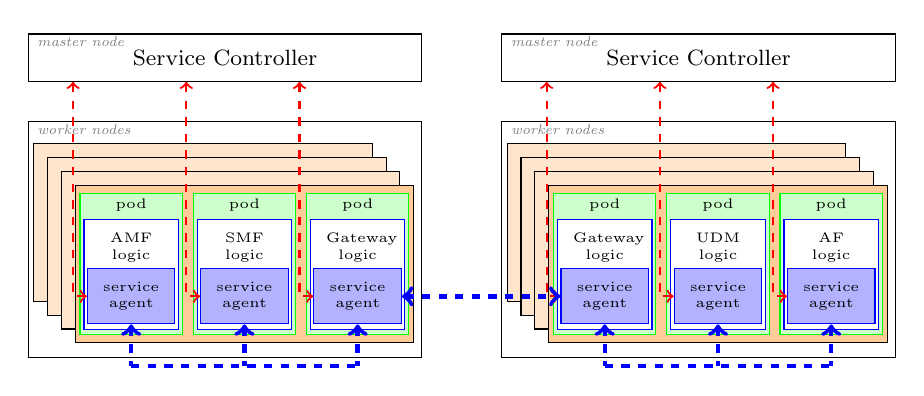
\begin{tikzpicture}[bound/.style={rectangle, draw=black,inner sep=0, fill=white, minimum width=5cm, minimum height=0.6cm,font=\footnotesize},
	cnode/.style={rectangle,draw=black,fill=orange!20, minimum width=4.3cm, minimum height=2cm},
	pod/.style={rectangle, inner sep=0, fill=green!20,draw=green, minimum width=1.3cm, minimum height=1.8cm},
	nf/.style={rectangle, inner sep=0, fill=white,draw=blue,minimum width=1.2cm, minimum height=1.4cm,above,yshift=2pt},
	agent/.style={rectangle, inner sep=3pt, fill=blue!30,draw=blue,text width=0.9cm, minimum height=0.7cm, font=\tiny, align=center},
	nflab/.style={text width=0.8cm,font=\tiny,align=center, inner sep=0},
	clink/.style={thick, red, dashed},
	dlink/.style={ultra thick, blue, dashed}]

		%controller
		\node[bound] at (0,0) (c1) {Service Controller};
		\node[bound,right] at ([xshift=1cm]c1.east) (c2) {Service Controller};
		\node[right] at ([yshift=-3pt]c1.north west) {\tiny \textcolor{black!50}{\textit{master node}}};
		\node[right] at ([yshift=-3pt]c2.north west) {\tiny \textcolor{black!50}{\textit{master node}}};
		%network functions
		\node[bound,minimum height=3cm,below] at ([yshift=-0.5cm]c1.south) (d1) {};
		\node[bound,minimum height=3cm,below] at ([yshift=-0.5cm]c2.south) (d2) {};
		\node[right] at ([yshift=-3pt]d1.north west) {\tiny \textcolor{black!50}{\textit{worker nodes}}};
		\node[right] at ([yshift=-3pt]d2.north west) {\tiny \textcolor{black!50}{\textit{worker nodes}}};

		\node[cnode,below] at ([yshift=-8pt,xshift=-8pt]d1.north) (n11) {};
		\node[cnode] at ([yshift=-5pt, xshift=5pt]n11) (n12) {};
		\node[cnode] at ([yshift=-5pt, xshift=5pt]n12) (n13) {};
		\node[cnode,fill=orange!40] at ([yshift=-5pt, xshift=5pt]n13) (n1) {};
		
		\node[cnode,below] at ([yshift=-8pt,xshift=-8pt]d2.north) (n21) {};
		\node[cnode] at ([yshift=-5pt, xshift=5pt]n21) (n22) {};
		\node[cnode] at ([yshift=-5pt, xshift=5pt]n22) (n23) {};
		\node[cnode,fill=orange!40] at ([yshift=-5pt, xshift=5pt]n23) (n2) {};
		\foreach \i in {1,2} {
			\node[pod] at ($(n\i.west)!0.1666!(n\i.east)$) (pod\i1) {};
			\node[pod] at ($(n\i.west)!0.5!(n\i.east)$) (pod\i2) {};
			\node[pod] at ($(n\i.west)!0.8333!(n\i.east)$) (pod\i3) {};
			\foreach \j in {1,2,3} {
				\node[below,yshift=-2pt,font=\tiny, inner sep=0] at (pod\i\j.north) {pod};
			}
		}
		
		\foreach \i in {1,2,3} {
			\node[nf] at (pod1\i.south) (nf1\i) {};
			\node[agent,above] at ([yshift=2pt]nf1\i.south) (agent1\i) {service agent};
			\node[nf] at (pod2\i.south) (nf2\i) {};
			\node[agent,above] at ([yshift=2pt]nf2\i.south) (agent2\i) {service agent};
		}
		\node[nflab,above] at ([yshift=2pt]agent11.north) {AMF logic};
		\node[nflab,above] at ([yshift=2pt]agent12.north) {SMF logic};
		\node[nflab,above] at ([yshift=2pt]agent13.north) { Gateway logic};
		\node[nflab,above] at ([yshift=2pt]agent21.north) {Gateway logic};
		\node[nflab,above] at ([yshift=2pt]agent22.north) {UDM logic};
		\node[nflab,above] at ([yshift=2pt]agent23.north) { AF logic};
		
		\foreach \i in {1,2} {
			\foreach \j in {1,2,3} {
				\draw[dlink,<-] (agent\i\j.south) -- ++ (0,-15pt);
				\draw[clink,<->] (agent\i\j.west) -- ++(-5pt,0) coordinate (ttp\i\j) -- (ttp\i\j |- c\i.south);
			}
		}
		\draw[dlink] ([yshift=-15pt]agent11.south) -- ([yshift=-15pt]agent13.south);
		\draw[dlink] ([yshift=-15pt]agent21.south) -- ([yshift=-15pt]agent23.south);
		\draw[dlink,<->] (agent13.east) -- (agent21.west);
	\end{tikzpicture}
  
  \caption{B5G integration fabric overall architecture  \label{fig1}}
  \end{center}
\end{figure*}

The architecture of the proposed fabric is based on Istio\cite{mesh}, a popular
cloud-native service mesh, with modifications to adapt to the SBA. It consists
of a centralized service controller and service agents which are illustrated on
the Figure \ref{fig1}. The NRF and SCP components in the original 5G
architecture is completely removed. Their roles of supporting a consumer to
select an appropriate instance of a target service within an application
context are realized by the service controller working in tandem with the
service agents.  In addition, common logic for NF discovery and selection
implemented at consumers are moved into the service agents. Any network
function is attached to an agent who acts as its proxy that do the request and
response on its behalf.  The agent abstracts away all the service
registration/discovery and selection from the signalling logic of the network
function.

However, concept of service agent in our fabric is different from the sidecar
proxy concept in existing cloud-native service meshes. An agent is a native
library that lives inside a network function. In the sidecar proxy models, an
agent lives in its own process. We opt for this approach in order to avoid the
latency incurred due to the full network protocol stack processing at sidecar
proxy agents. In addition, the service discovery protocol among agents and
controller also needs to be designed differently to reflect the complexity of
service identification in mobile core network (see Section \ref{sec:nf-id}).

In order to support deployments that span across multiple domains, such as the
cases of multi-domain slicing, we introduce a new network function named
service gateway. A gate to connect its domain to other gateways in other
domains. Similar to the others network function, it is built upon the service
agent and received routing rules from the service controller to forward
requests and responses across domains. When an agent has an request that
targets a cross-domain service, the request is forwarded to a gateway toward
the target domain cluster.

\subsection{Fabric composition}


\begin{figure}
\begin{center}
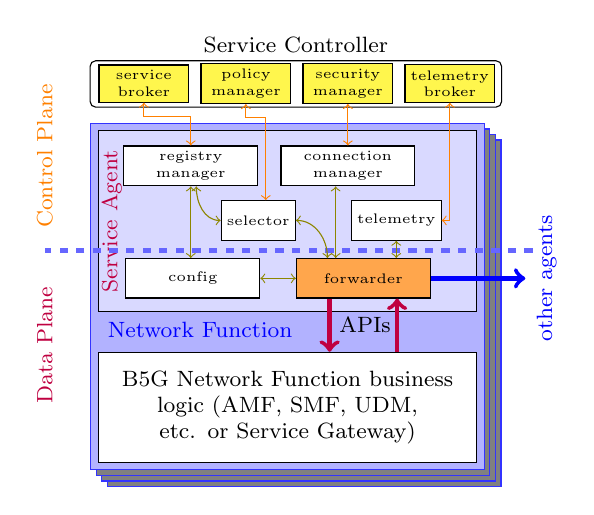
\begin{tikzpicture}[comlab/.style={font=\tiny\linespread{0.6},align=center,inner sep=2pt},
ccom/.style={rectangle,draw=black,fill=yellow!70,text width=1cm},
dcom/.style={rectangle,draw=black,fill=white, minimum height=0.5cm},
nf/.style={rectangle,draw=blue!80,fill=black!50,minimum width=5cm,minimum height=4.4cm}]
	%network functions
	\node[nf] at (0,0) (nf4) {};
	\node[nf] at ($(nf4)+(-2pt,2pt)$) (nf3) {};
	\node[nf] at ($(nf3)+(-2pt,2pt)$) (nf2) {};
	\node[nf,fill=blue!30] at ($(nf2)+(-2pt,2pt)$) (nf1) {};

	%controller
	\draw[rounded corners=2pt,fill=white] ([yshift=0.2cm]nf1.north west) rectangle ([yshift=1cm]nf4.north east);
	\node[font=\footnotesize] at ([yshift=1.1cm]$(nf1.north west)!0.5!(nf4.north east) $){Service Controller};
	\node[comlab,ccom,right] at ([yshift=0.5cm,xshift=3pt]nf1.north west) (c1) {service broker};
	\node[comlab,ccom,right] at ([xshift=4pt]c1.east) (c2) {policy manager};
	\node[comlab,ccom,right] at ([xshift=4pt]c2.east) (c3) {security manager};
	\node[comlab,ccom,right] at ([xshift=4pt]c3.east) (c4) {telemetry broker};
	%nf logic
	\node[minimum width=4.8cm, minimum height=1.4cm, fill=white, draw=black] at ([yshift=0.8cm]nf1.south) (nfb){};
	
	\node[text width=4.5cm, inner sep=4pt, align=center,font=\footnotesize] at (nfb) {B5G Network Function business logic (AMF, SMF, UDM, etc. or Service Gateway)};
	\node[font=\footnotesize,blue,right] at ([yshift=8pt]nfb.north west) {Network Function};	
	%agent
	\node[minimum width=4.8cm, minimum height=2.3cm, fill=blue!15, draw=black,above] at ([yshift=0.5cm]nfb.north) (ag){};
	\node[rotate=90,font=\footnotesize,purple] at ([xshift=5pt]ag.west) {Service Agent};
	
	\node[dcom, comlab, above, minimum width=1.7cm] at ([yshift=5pt]$(ag.south west)!0.25!(ag.south east)$) (conf) {config};
	\node[dcom, comlab, fill=orange!70, above,minimum width=1.7cm] at ([yshift=5pt]$(ag.south west)!0.7!(ag.south east)$) (fwd) {forwarder};
	\node[dcom, comlab, below,minimum width=1.7cm, text width=1.5cm] at ([yshift=-15pt]c3.south) (sec) {connection manager};
	\node[dcom, comlab, left, minimum width=1.7cm, text width=1.5cm] at ([xshift=-8pt]sec.west) (disc) {registry manager};

	\node[dcom, comlab, below] at ([yshift=-5pt]disc.south east) (sel) {selector};
	\node[dcom, comlab, right] at ([xshift=0.7cm]sel.east) (tel) {telemetry};
	
	\draw[<->,orange] (c1.south) -- ++(0,-5pt) -| (disc.north);
	\draw[<->,orange] (c2.south) -- ++(0,-5pt) -| ($(sel.north west)!0.6!(sel.north east)$);
	\draw[<->,orange] (c3.south) -- (sec.north);
	\draw[<->,orange] (c4.south)  |- (tel.east);
	\coordinate (p1) at ($(fwd.south west)!0.25!(fwd.south east)$);
	\coordinate (p2) at ($(fwd.south west)!0.75!(fwd.south east)$);
	\draw[->,ultra thick, purple] (p1) -- node (apilab) {} (p1 |- nfb.north);
	\node[right] at (apilab) {\footnotesize APIs};
	\draw[<-,ultra thick, purple] (p2) -- (p2 |- nfb.north);
	\draw[->,ultra thick, blue] (fwd.east) -- +(1.2cm,0) node[below, rotate=90, align=center] (p3) {\footnotesize other agents};
	\draw[ultra thick, blue!60, dashed] ($(p3)+(-5pt, 10pt)$) -- ++(-6.2cm,0) coordinate (p4);
	\node[rotate=90,orange] at ([yshift=1.2cm]p4) {\footnotesize Control Plane};
	\node[rotate=90,purple] at ([yshift=-1.2cm]p4) {\footnotesize Data Plane};
	\draw[olive,<->] ([xshift=2pt]disc.south) to[out=-90,in=180] (sel.west);
	\draw[olive,<->] (disc.south) -- (disc.south |- conf.north);
	\draw[olive,<->] (conf.east) -- (fwd.west);
	\draw[olive,<->] (tel.south) -- (tel.south |- fwd.north);
	\coordinate (fwd1) at ([xshift=-10pt]fwd.north);
	\coordinate (fwd2) at ([xshift=-3pt]fwd1);
	\draw[olive,<->] (fwd1) -- (fwd1 |- sec.south);
	\draw[olive,<->] (fwd2) to[out=90,in=0] (sel.east);
\end{tikzpicture}

\end{center}
\caption{Functional components of the proposed B5G integration fabric}
\label{fig2}
\end{figure}

In this section, we further detail the composition of the fabric by dissecting
it into smaller components to describe their roles and interactions. The
composition is shown on Figure \ref{fig2}. At the top is the service controller
which consists of four components in yellow color. The lower blue boxes
represent network functions.

A network function composes of its business logic part and a service agent.
The service agent provides APIs for requesting service and responding to
requests. The agent executes service discovery and selection and hides these
procedures from the business layer. The agent therefore belongs to both control
plane and data plane. On the data plane, it routes request/response toward
other agents. On the control plane, it interacts with the service controller to
dynamically update internal routing rules.

The \textit{forwarder} is the core module of the service agent on the data
plane part. On one hand, it interfaces with the business logic part to handle
its requests and responses. On the other hand, it maintains a list of transport
connections to the other service agents to forward outgoing and receiving
incoming requests and responses. The \textit{config} component keep
information that defines how the service agent should behave. It may have a
list of static connection information to other service agents, a default policy
to select a network function from a list of candidates.

The \textit{registry manager} component implements all procedures for
notifying of the network function to the fabric and discovery other network
functions of interests. It interacts with the \textit{service broker} component
of the service controller to keep synchronizing with the whole mesh. When the
\textit{forwarder} needs to forward a request to a new remote service, it asks
the \textit{registry manager} component for a list of candidate
locations of the target service then selects one of the candidate to make a
connection for sending the request. The \textit{selector} component implements
load balancer algorithms to make the selection. It is the \textit{policy
manager} component at the service controller that chooses the load balancing
algorithm to be used at the service agent.

The \textit{connection manager} component at the service agent cooperates with
the \textit{security manager} at the service controller to create secured
connections between service agents. The \textit{security manager} might
generate a private key and sign a corresponding certificate for the agents and
distributes the certificate to the agents. The agents then use the information
to establish secured connections for delivering the data plane traffic.

Finally, the \textit{telemetry} component at the agent and the
\textit{telemetry broker} component at the controller provides the
observability for the fabric. Since all the signalling traffic among network
functions is channeled through the service agents, the \textit{telemetry}
component might collect statistics of the traffic, then make them available for
serving to the network. The \textit{telemetry manager} specifies what
telemetric data to be collected at the agents and it may also pull the data
from them for data analytics.


\subsection{Identifying a network function\label{sec:nf-id}}

In the cloud-native method of deployment, each service is identified with a
long-lived name that exists uniquely within the namespace of its application.
It is the service mesh that maintains a mapping of the name to locations of its
deployed instances. Multiple instances of the same service can be deployed and
the service mesh selects the best one to serve a request. Business logic of the
application therefore is constructed using service names instead of locations
of their deployed instances.

However, a service in 5G core network, albeit having a name, must be identified
with an NF serving it. In order to separate the mobile signaling logic from NFs
deployment there must be a mechanism to maintain persistent identifications of
NFs. This is to enable the fabric to map an NF identification to locations of
its deployed instances. 

It is hardly possible to assign a static name to an NF. The reason is that an
NF may operate in multiple application scopes. The following example explains
this complexity.  Suppose that there is an terminal UE$_1$ operating in a slice
\textit{slice-a} in a domain \textit{example.domain}, signaling procedures
relevant to UE$_1$ may refer to an AMF (Access and Mobility Function) by an
unique name as \textit{/example.com/slice-a/amf}.  However, if the same AMF can
also operate in a slice \textit{slice-b}, and there is an terminal UE$_2$ that
needs access to both slices at the AMF, then it is not possible to assign the
AMF a unique name.

Therefore, in order to look for a specific producer in a signalling procedure,
a consumer has to specify a list of criteria and query the NRF for suitable
candidates (see section 6.3 / TS 23.501\cite{rel16}). The NRF only responses to
requests which conform to the standard, that is, the list of valid criteria is
pre-defined. This raises an issue: it is not possible to include new types of
NFs because they are not recognisable by the NRF. It limits the possibility of
network expansion to adopt new use cases.

Our fabric is designed with openness to accept new types of NFs.  This is to
support the vision that a network operators should be able to integrate any new
applications into their networks without making changes to their existing
infrastructure. Service components of a new application can register themselves
with the fabric so that their supported services can be routed seamlessly among
them following the application's programmed logics.

For realizing this scheme, we introduce the concept of application context. It
is defined as a logical setting where a group of network functions may interact
to make sense of certain application logic. Examples may include a PLMN, a
DNN, a network slice, or a network slice instance, etc. These are the
pre-defined context in the 5G specification. However, there is no restriction
on the list of valid contexts. A network operator should be free to define new
contexts according to the need of new applications.

Within a context relevant to an application, there can be multiple instances of
a network function being deployed. From the perspective of the application,
they are identical, thus, can be called upon interchangeably. For example,
deployed instances of the AMF within a slice are identical in term of handling
signaling procedures in that slice.

A primitive context $C$ can be represented as a key-value pair $(C^k, C^v)$
where $C^k$ is the context identity which defines a primitive type of context,
while $C^v$ is a value of that type. A new context can be created by taking
intersection of a set of existing contexts: $C = \bigcap_{i=1}^{n}{C_i}$.
Alternatively, that same context can be represented as a list of key-value
pair: $C=\{(C_i^k, C_i^v)\}$.  

When a consumer needs to find a producer to request a service in a certain
context, it sends a list of key-value pairs representing the context and the
type of producer to the fabric. With that provided information, the fabric
should be able to identify all currently deployed instances of that producer.
It then chooses one of them as a destination to forward the consumer's request.

\subsection{Agent to NF's business logic  interface}
\begin{figure}
\begin{center}
	\includegraphics[width=0.4\textwidth]{api}
	\caption{A sample code of requesting a service\label{fig:api}}
\end{center}
\end{figure}

With the introduction of application context concept, it is now simple to
define the interface exposed by the agent library to the business layer of a
NF. Figure \ref{fig:api} presents a sample code (without error
handling) to describe the flow of service requesting to a producer.

When the NF is initiated, it first creates  an \textit{agent} object  (line 3)
with certain configuration parameters (loaded from a configuration file by the
\textit{configuration} module). At creating time, the agent starts
(under-the-hood) to register itself to the integration fabric for other agents
to request its services.

While being in a signaling procedure, the NF may want to request a service from
a producer, it first builds a context to express the identification of the
producer (line 6). It then requests the agent to find the target by providing
the list and the type of producer (line 7). Transparently, the agent should
proceed discovery and selection process and returns to the caller a connection
object (\textit{conn}) that represents a transport connection to the selected
producer. The connection is persistent to request services in multiple times
(line 9-20). 

\subsection{Distributed service registry}

\begin{figure}[h]
\begin{center}
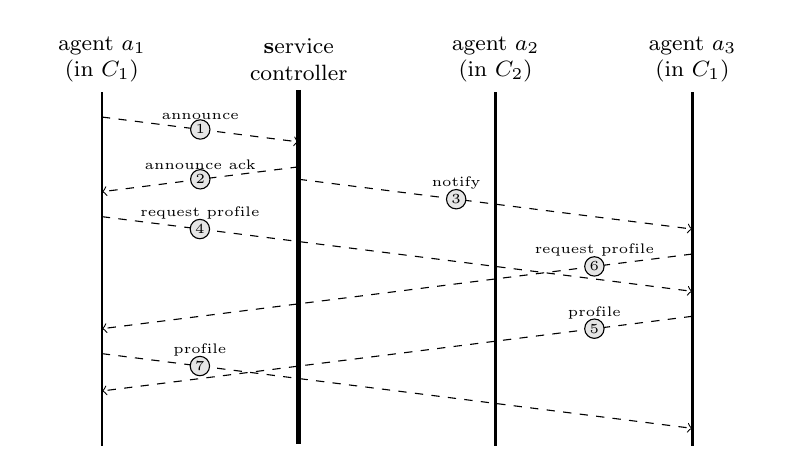
\begin{tikzpicture}[lab/.style={font=\footnotesize\linespread{0.8},text
	width=1.65cm,align=center},
axis/.style={thick},
link/.style={->, dashed},
linklab/.style={draw,circle,minimum width=7pt,fill=black!10,inner sep=0,font=\tiny},
msg/.style={above,font=\tiny}]
	\def\xx{2.5cm}
	\def\yy{-9pt}
	\def\ll{-4.5cm}
	\node[lab] at (0,0) (f1) {agent $a_1$ (in $C_1$)};
	\node[lab] at ([xshift=\xx]f1) (f2) {\textbf service controller};
	\node[lab] at ([xshift=\xx]f2) (f3) {agent $a_2$ (in $C_2$)};
	\node[lab] at ([xshift=\xx]f3) (f4) {agent $a_3$ (in $C_1$)};	

	\draw[axis] (f1.south) -- +(0,\ll);
	\draw[axis, ultra thick] (f2.south) -- +(0,\ll);
	\draw[axis] (f3.south) -- +(0,\ll);
	\draw[axis] (f4.south) -- +(0,\ll);

	%register
	\draw[link] ([yshift=\yy]f1.south) -- node (l1) {} ++(\xx,\yy) coordinate (p1);
	%response
	\draw[link] ([yshift=\yy]p1) -- node (l2) {} ++(-\xx,\yy) coordinate (p2);
	%notify
	\draw[link] ([yshift=1.5*\yy]p1) -- node[pos=0.4] (l3) {} ++(2*\xx,2*\yy) coordinate (p3);
	%pull
	\draw[link] ([yshift=\yy]p2) -- node[pos=0.166] (l4) {} ++(3*\xx,3*\yy) coordinate (p4);
	%pull-response
	\draw[link] ([yshift=\yy]p4) -- node[pos=0.166] (l5) {} ++(-3*\xx,3*\yy) coordinate (p5);
	
	\draw[link] ([yshift=\yy]p3) -- node[pos=0.166] (l6) {} ++(-3*\xx,3*\yy) coordinate (p6);
	%pull-response
	\draw[link] ([yshift=\yy]p6) -- node[pos=0.166] (l7) {} ++(3*\xx,3*\yy) coordinate (p7);
	
	\foreach \i in {1,...,7} {
		\node[linklab] at (l\i) {\i};
	}
	\node[msg] at (l1) {announce};
	\node[msg] at (l2) {announce ack};
	\node[msg] at (l3) {notify};
	\node[msg] at (l4) {request profile};
	\node[msg] at (l5) {profile};
	\node[msg] at (l6) {request profile};
	\node[msg] at (l7) {profile};a network function can
discovery the location of a service quickly because its co-located agent keeps
necessary registry data.

\end{tikzpicture}
\caption{Distributed service registration flow}
\label{fig3}
\end{center}
\end{figure}

The introduction of the integration fabric with unified APIs that separates
service implementation and service deployment enables various methods for
realizing service discovery and selection. In this work, we propose a
distributed service registry platform that is more responsive and more scalable
than current NRF-based method.

In this approach, the full service registry database is not kept at a
centralized entity. Instead, it is distributed to service agents of NFs. Each
agent only manages a partial registry which holds records of services of
certain relevant contexts. The service controller works as a broker to notify
the agents of registration updates in a selective manner.  This approach
removes the bottleneck issue of the NRF-based method. In addition, discovery
becomes much more responsive as the agent (having registry records) is co-located
with the consumer.

Figure \ref{fig3} illustrates a common procedure of service registration and
registry update at agents. In the example, there are three agents: $a_1$ is
newly initiated and it needs to announce its existence to the fabric while the
other two ($a_2$ and $a_3$)  already announced. Suppose that current deployment
has two context $C_1$ and $C_2$. The agent $a_1$ and $a_3$ are operating in
$C_1$ while the agent $a_2$ is operating in $C_2$.

When the network function instance $nf_1$ attached to the agent $a_1$ is
initiated, the agent itself announces to the service controller (path
\tikz{\node[circle, draw, minimum width=6pt,inner sep=0,font=\tiny] at (0,0)
{1};}). The agent is configured to know the address of the controller.  The
announcement includes following pieces of data: a) the transport address of the
agent; b) a list of primitive contexts ($L_o = \{C_1\}$) where $nf_1$ operates;
c) and a list of primitive contexts of $nf_1$'s concerning ($L_i = \{C_1\}$).
The list $L_i$ is to express to the controller the intention of $nf_1$ to which
contexts it wants to listen for registration updates. 

The service controller maintains a list of announced agents; and it also keeps
track of their contexts as well as the contexts they wish to monitor.

Upon receiving the request, the controller responses (path \tikz{\node[circle,
draw, minimum width=6pt,inner sep=0,font=\tiny] at (0,0) {2};}) with a list of
locations of agents which belong to the interested contexts that was expressed
by the requester. For example, $a_1$ includes context $C_1$ in its interested
list, the controller should include the address of $a_3$ the response.

At the same time, the controller notifies (path \tikz{\node[circle, draw,
minimum width=6pt,inner sep=0,font=\tiny] at (0,0) {3};}) all agents $C_1$ of
the new registration. The agent $a_3$ should receive the notification (supposed
that it has also expressed an interest in $C_1$'s updates).

The agent $a_1$ extracts the list of announced agents in the response from the
controller, then sends a request to each of them for retrieving their profiles
(path \tikz{\node[circle, draw, minimum width=6pt,inner sep=0,font=\tiny] at
(0,0) {4};}). Similarly, the agent $a_3$ also sends a request to $a_1$ to pull
its profile (path \tikz{\node[circle, draw, minimum width=6pt,inner
sep=0,font=\tiny] at (0,0) {6};}). Upon receiving a request, a receiving agent
should respond with its profile (path \tikz{\node[circle, draw, minimum
width=6pt,inner sep=0,font=\tiny] at (0,0) {5};} and \tikz{\node[circle, draw,
minimum width=6pt,inner sep=0,font=\tiny] at (0,0) {7};} ).



\section{Conclusion\label{sec:conc}}

In this work, we analyzed the current 5G core network architecture and
identified its limitations in terms of realizing a cloud-native deployment. We
proposed a separation of control plane and data plane in the signaling network.
Specifically, NFs interacts in the data plane to fulfil the signaling
procedures of mobile applications. However, how the signaling traffic is
forwarded on the data plane is specified by the control plane. It is the
network operators that configure and program the control plane to meet their
deployment requirements.

For envisioning the concept we introduced an integration fabric and explained
how it is composed. The two network functions NRF and SCP which were originated
from the 5G architecture are merged to become a service controller of the
fabric. Common procedures within other NFs for service discovery and routing
will be implemented in a service agent library. A simplified set of APIs
between business layer of NFs and the service agents is introduced to turn the
fabric into a black-box which allows the NFs can be developed without
concerning of how they are deployed and scaled.

The separation allows us to explore different approaches for realizing the
control plane of the fabric. We proposed a distributed service discovery
framework where service registry is managed partially at each service agent.
The service controller plays the role of a registry broker. It notifies updates
of services to the agents which are interested. Our approach brings two
advantages: first, traffic congestion at the centralized registry (NRF) is
removed as the registry is now distributed across agents; second, discovery of
a producer can be instantly fast as necessary registry data is now localized
at consumer's agent.

We are currently in-progress of detailed design and implementation of the
proposed integration fabric. The free5gc\cite{free5gc}, an open-source 5G core
network implementation, is used as a codebase to integrate the service agent
library of the fabric. We are planing to build a test-bed environment on
multiple clouds using Kubernetes with our fabric to verify the architecture in
realizing large-scale deployments of cross domains network slicing use cases to
support vertical applications.

\section*{Acknowledgment}

This work was supported by the ICT R\&D program of MSICT/IITP. [2021-0-02094,
International collaborative research on 6G network architecture and core
technologies]

%\section*{References}

\begin{thebibliography}{00}
\bibitem{5g} Gupta, Akhil, and Rakesh Kumar Jha. ``A survey of 5G network: Architecture and emerging technologies.`` IEEE access 3 (2015): 1206-1232.
\bibitem{telco} Alliance, N. G. M. N. ``Cloud Native Enabling Future Telco Platforms.`` (2021).
\bibitem{ku8} Luksa, Marko. ``Kubernetes in action``. Simon and Schuster, 2017.
\bibitem{kube5g} Arouk, Osama, and Navid Nikaein. ``Kube5g: A cloud-native 5g service platform.`` GLOBECOM 2020-2020 IEEE Global Communications Conference. IEEE, 2020.
%\bibitem{5gproc} 3GPP. ``Procedures for the 5G system (5GS)(release 16): TS 23.502.`` (2020).
\bibitem{rel15} 3GPP. ``System architecture for the 5G system (5GS).`` 3rd Generation Partnership Project (3GPP), Technical Specification (TS) 23.501 (2018).
\bibitem{rel16} 3GPP. ``System architecture for the 5G system (5GS).`` 3rd Generation Partnership Project (3GPP), Technical Specification (TS) 23.501 (2020).
\bibitem{huawei} Huawei. ``5G Signaling and Control Plane Traffic Depends on Service Communications Proxy (SCP)``, Whitepaper, 2021.
\bibitem{oracle} Oracle. ``Managing 5G signalling complexity``, Whitepaper, Oracle Communications, 2021.
\bibitem{mesh} W. Li et al., ``Service Mesh: Challenges State of the Art and Future Research Opportunities``, 2019 IEEE Int'l. Conf. Service-Oriented System Engineering, pp. 122-25, 2019.
\bibitem{free5gc} Free5GC, ``free5GC: an opensource 5G core network``, \url{https://www.free5gc.org}, 2022.
\end{thebibliography}

\end{document}
